\section{Application Structure}

The structure of \projectname{} is a bit different from other web applications.

\subsection{Architecture}

The architecture of \projectname{} differs from other web applications in the way that there exists two different type of servers. The server where the web application is running is called Master after this denoted M.
For each drone in the system there is a Slave denoted S. 
On both M and S there exists daemons which is responsible for different tasks, however there is some similarity that is that these tasks can happen at anytime therefore the program needs to be running at anytime. These daemons are denoted D.
Each user have a browser they view the application through this is denoted B.
It is M's responsibility to communicate with every S in the system.
S is responsible for all communication with the drone it is parred with.

When a new S appears in the system

\begin{figure}[htb]
    \centering 
    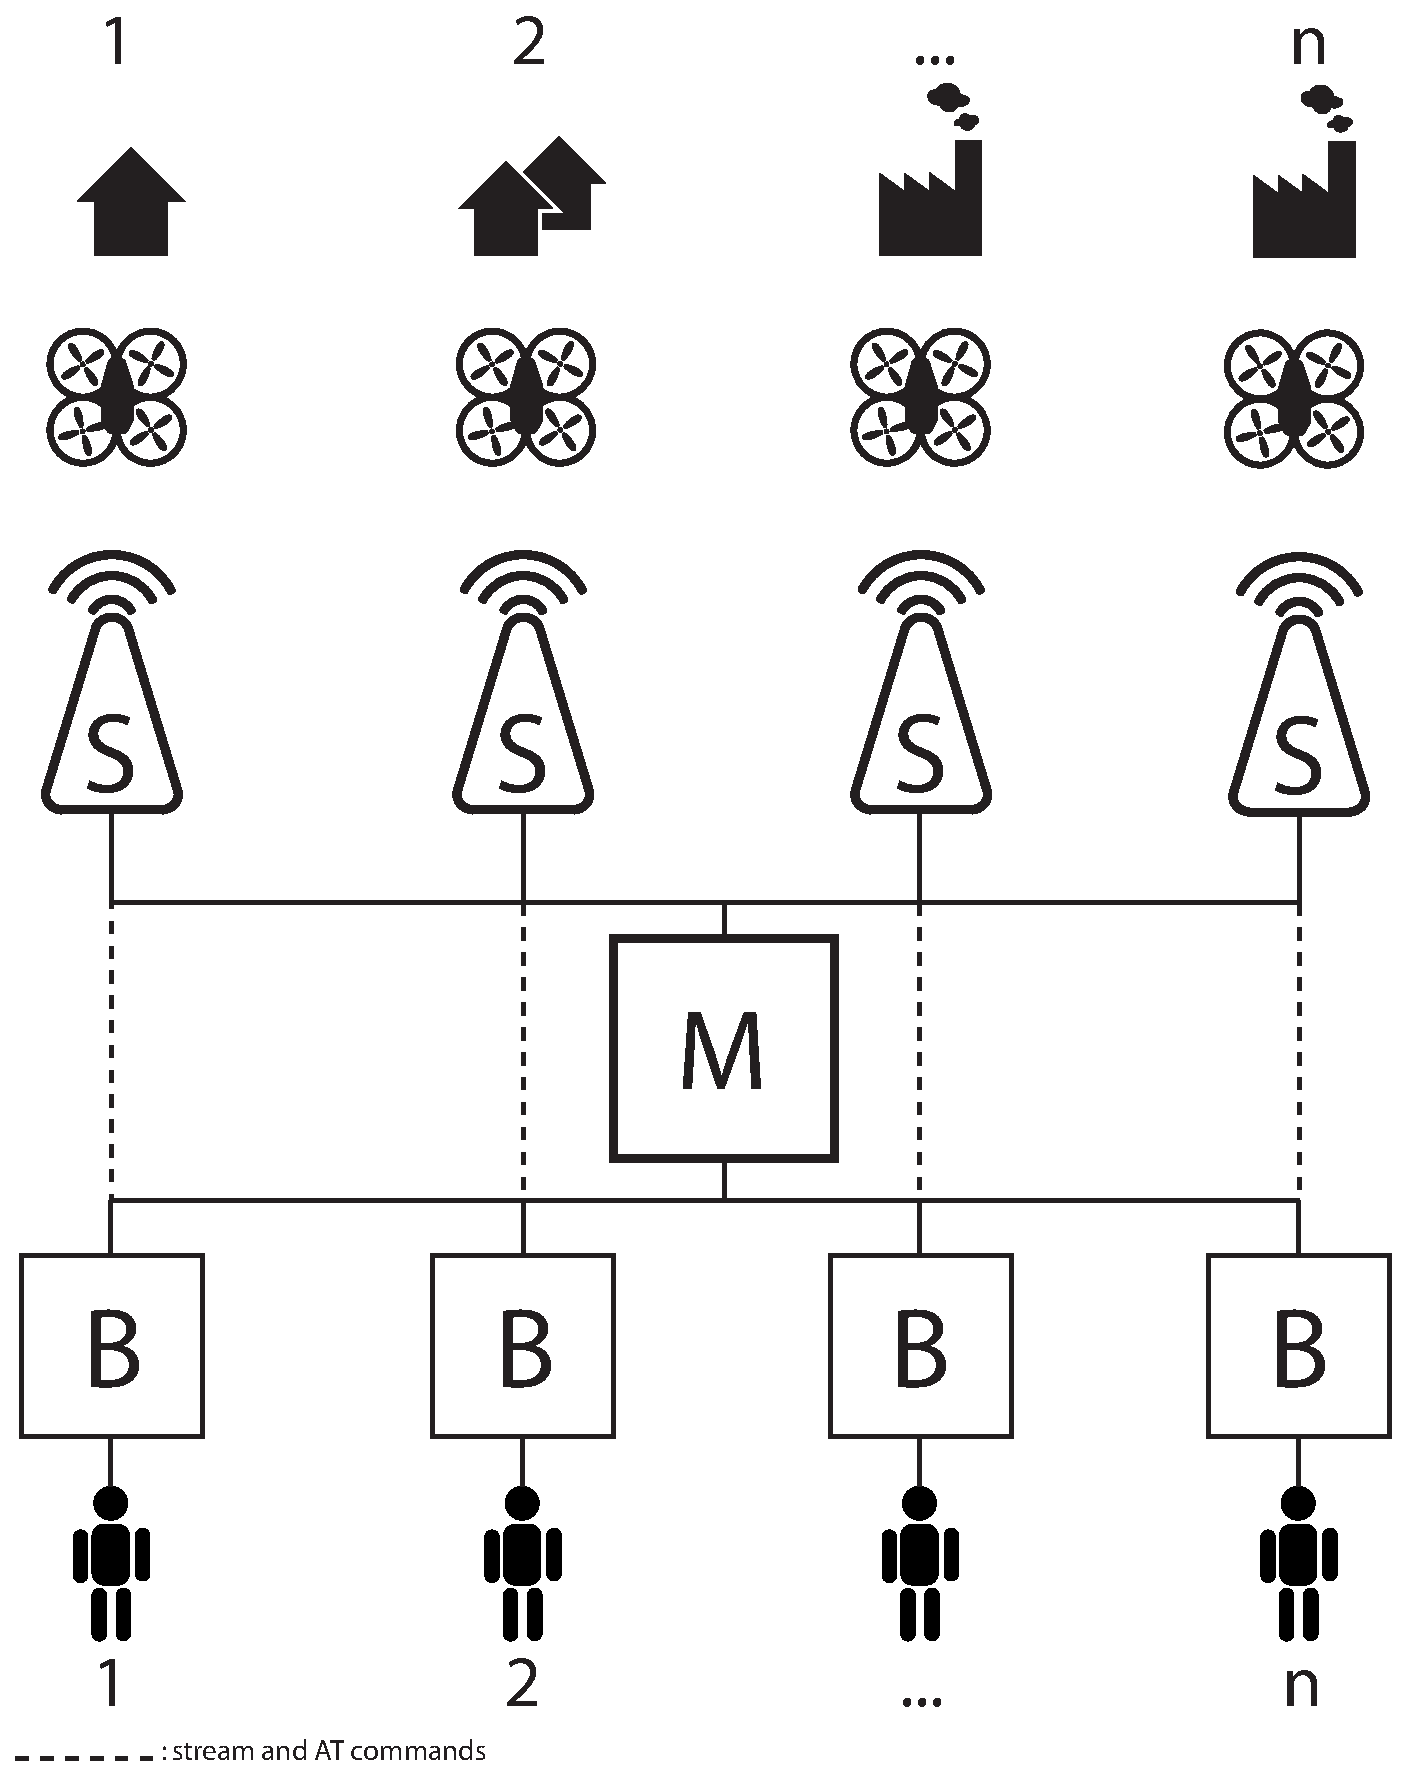
\includegraphics[width=\textwidth]{gfx/system_architecture.pdf}
    \caption{System architecture of \projectname{}}
    \label{fig:system_architecture}
\end{figure}


(Why is this different from other web applications)

\subsection{Master M}

(Only one M?)

\subsection{Slave S}

(More S's?)

\subsection{Daemons}

